\documentclass{scrartcl}
\usepackage{handout}
\usepackage{booktabs, multirow} % for borders and merged ranges
\usepackage{soul}% for underlines
\usepackage[table]{xcolor} % for cell colors
\usepackage{changepage,threeparttable} % for wide tables

% \usepackage[garamond]{mathdesign}
\usepackage{pgfplots,pgf-pie, multirow}
\pgfplotsset{width =15cm,compat=1.9}
\usepackage{tikz,enumitem}
 
\setlength{\tabcolsep}{10pt}
\setlength{\arrayrulewidth}{0.6pt}
\renewcommand{\arraystretch}{1.175}
 
\title{Behaviour of Ants Observed using different techniques}
\author{Sabarno Saha (22MS037)}
\date{\today}
\newpage
\begin{document}
\maketitle
\tableofcontents
\newpage
\section{Aim}
\begin{enumerate}
    \item To identify all individuals uniquely using their color codes
    \item To quantify the proportion of active/inactive individuals using scan sampling
    \item To quantify the work-load of leaders during tandem-run using focal sampling
\end{enumerate}
\section{Theory}
We are undertaking the project of observing behavioural observations of ants \textit{Diacamma Indicum}. 
\textit{Dicamma Indicum} is type of ant found in India, Sri Lanka and Japan. We define 
\textbf{behaviour} as an action or a series of actions exhibited by an organism in response to 
a particular environment or a change. In this experiment we observe Tandem running. 
\textbf{Tandem Run} is pairwise coordinated movement observed in ants and termites. 
Ants use tandem runs for social learning. An ant leads another native ant from the nest to 
the new source it has found. A tandem run consists of a leader and a follower. The follower ant 
maintains contact with the leader ant by frequently touching the leader's legs and abdomen 
with its antennae.
\section{Methods}\label{meth}
Behavioural sampling can be done in multiple ways namely,
\begin{itemize}
    \item \textbf{Ad Libitum} We note whatever is visible at a certain time. The data is not taken systematically.
    \item \textbf{Scan Sampling} Here we break the entire time interval of observations into smaller timeframes. In each timeframe we observe the activity of individuals.
    \item \textbf{Focal Sampling} Here we focus on a certain indivual or unit or a certain behaviour. We can have focal animal samling where a particular individual is fcused on during the whoe observation time to see its behaviour. We also hav focal behaviour sampling where we observe a certain behaviour of the individuals throughout the observation time.
\end{itemize}
First we will go through the whole video to identify all the ants uniquely using their given color codes. This is
done ad libitum, as we watch through the whole video.
For this experiment, we have a video of 41 mins and 19 seconds. We will use scan sampling to see what 
the ants are doing at intervals of 3 mins, so around 13-14 samplings. We will record using scan sampling 
the activity of the ants i.e. if they are running or stationary during the scan samples and where they are 
located namely in the nest, around the door to the nest or on the track. 
We will then use focus sampling to identify tandem runs and their frequency corresponding to the ants.
Then we will see if those ants have heavy or light workload, as per the average number tandem runs as the 
threshold.
\subsection{Coloring}
The ants are coloured in three places, the head, the thorax and the abdomen. If any one of these three 
is uncolored, we put a blank(-) there. The colors are y for yellow, b for blue, r for red and w for white. 
For example if we write 'y-b', we mean yellow on the head, no paint on the thorax, and blue on the abdomen.
\subsection{Scan sampling}
We will identify what the ants are doing using scan sampling. We break the video in 3min chunks and 
then identify what the ants are doing. They are classified into active vs inactive ants. We move 
1 second back and front. If they are not moving in that time interval, they will be classified as inactive.
Otherwise they will be classified as active. They are then classified based on location, on whether 
they are on the track, near the nest door, or inside the nest.

\section{Observations}
\subsection{List of Unique ants}
We observed the entire video and noted all ants we saw(ad libitum) throughout the video. Then the 
total ants are run through a python program to select all the unique ones. We obtain a total of
\textbf{33 unique individuals}. Some colours were not properly visible and unclear individuals were noted 
twice throughtout the video. Along with the \textbf{33 unique individuals}, we also have \textbf{2 unclear instances}
 of ants. So we have atleast \textbf{34 unique individuals}.
\begin{table}[H]
        \centering
\begin{tabular}{|p{0.75in}|p{1.25in}|}
\hline 
 Sl No. & Unique individuals \\
\hline 
 1 & y-y \\
\hline 
 2 & b-y \\
\hline 
 3 & -y- \\
\hline 
 4 & yww \\
\hline 
 5 & -yy \\
\hline 
 6 & wy- \\
\hline 
 7 & w-w \\
\hline 
 8 & -wy \\
\hline 
 9 & by- \\
\hline 
 10 & --y \\
\hline 
 11 & -yb \\
\hline 
 12 & -ww \\
\hline 
 13 & yyw \\
\hline 
 14 & --r \\
\hline 
 15 & yy- \\
\hline 
 16 & yw- \\
\hline 
 17 & wyy \\
\hline 
 18 & -bb \\
\hline 
 19 & -yw \\
\hline 
 20 & wwy \\
\hline 
 21 & ww- \\
\hline 
 22 & w-- \\
\hline 
 23 & -w- \\
\hline 
 24 & w-y \\
\hline 
 25 & www \\
\hline 
 26 & --b \\
\hline 
 27 & -wr \\
\hline 
 28 & --w \\
\hline 
 29 & y-w \\
\hline 
 30 & yyy \\
\hline 
 31 & wyw \\
\hline 
 32 & yyb \\
\hline 
 33 & y-b \\
 \hline
\end{tabular}
\end{table}
\subsection{Scan Sampling}
We classify scan sampled ants into active or inactive ants. The way we classify ants into active and 
inactive ants have been detailed out in the \nameref{meth}. We also identify where the ants are present 
while taking the scans. The locations are labelled into \textbf{1. Track 2. Near the nest door 3. In the nest}.
We also take some special behaviours into concern while taking scans.
\begin{adjustwidth}{-2.5 cm}{-2.5 cm}\centering\begin{threeparttable}[!htb]
\scriptsize
\begin{tabular}{lrrrrrrr}\toprule
Sl no &Time(in min) &Individual &Active/Inactive &Location &Special Behaviour & \\\midrule
1 &0 &No ant &- &- &- & \\
2 &3 &No ant &- &- &- & \\
3 &6 &No ant &- &- &- & \\
4 &9 &No ant &- &- &- & \\
5 &12 &y-w &Active &Inside the Nest &Minimal movement in the nest & \\
6 &15 &wwy &Inactive &Inside the Nest &- & \\
7 &18 &No ant &- &- &- & \\
8 &\multirow{5}{*}{21} &-yy &Inactive &On Track &Very restricted movement & \\
9 & &wwy &Inactive &On Track &- & \\
10 & &-wy &Active &Nest Door &Entering the nest door & \\
11 & &-y- &Active &Nest Door &Entering the nest door carrying an egg & \\
12 & &Unclear &Inactive &Nest Door &- & \\
13 &\multirow{3}{*}{24} &y-w &Active &On track &Leader of a tandem run & \\
14 & &-yb &Active &On track &Follower of the tandem run & \\
15 & &Unclear &Active &Nest Door &Moving around the nest door & \\
16 &\multirow{3}{*}{27} &-yw &Active &Nest Door &Coming out of the nest & \\
17 & &ww- &Inactive &Inside the Nest &- & \\
18 & &b-y &Inactive &Inside the Nest &- & \\
19 &\multirow{2}{*}{30} &yww &Inactive &Nest Door &- & \\
20 & &-yw &Active &On track &Moving away from the nest & \\
21 &\multirow{3}{*}{33} &-yy &Inactive &Nest Door &- & \\
22 & &-w- &Active &Nest Door &Entering the nest & \\
23 & &Unclear &Active &Track &Moving towards the nest & \\
24 &\multirow{2}{*}{36} &-yw &Active &Nest Door &Entering the nest door & \\
25 & &yww &Active &Inside the Nest &Moving around inside the nest & \\
26 &\multirow{4}{*}{39} &www &Active &Inside the Nest &- & \\
27 & &-yw &Inactive &Nest Door &Very restricted movement & \\
28 & &-w- &Inactive &Nest Door &- & \\
29 & &wwy &Active &Track &Very restricted movement towards the nest door & \\
30 &41 &-y- &Inactive &Inside the Nest &- & \\
\bottomrule
\end{tabular}
\end{threeparttable}
\end{adjustwidth}
\newpage

\subsection{Tandem Runs}
Here is a list of all tandem runs observed throughout the whole video.
\begin{table}[H]\centering
\scriptsize
\begin{tabular}{lrrrr}\toprule
Sl No. &Leader &Follower &Comments \\\midrule
1 &y-w &y-b & \\
2 &y-w &wwy & \\
3 &y-w &--y & \\
4 &-wy &wy- & \\
5 &wwy &Unclear & \\
6 &-yw &wy- & \\
7 &y-w &www & \\
8 &w-y &y-y & \\
9 &wwy &-yw & \\
10 &-wy &-y- & \\
11 &y-w &Unclear & \\
\multirow{2}{*}{12} &www &-yb &\multirow{2}{*}{One single tandem runs with three ants} \\
&www &-wy & \\
13 &y-w &wyw & \\
14 &www &ww- & \\
15 &wwy &-bb & \\
16 &y-w &-ww & \\
17 &-wy &yyy & \\
\multirow{3}{*}{18} &y-w &wy- &\multirow{3}{*}{Part of one tandem run with 4 ants} \\
&wy- &www & \\
&www &-bb & \\
19 &y-w &--b & \\
20 &wwy &yyb & \\
21 &-wy &w-w & \\
22 &y-w &-yb & \\
23 &www &--y & \\
24 &wwy &--r & \\
25 &yw- &w-- & \\
26 &www &b-y & \\
27 &y-w &w-y & \\
28 &wwy &--b & \\
29 &-wy &wyy & \\
30 &wwy &yw- & \\
31 &y-w &-w- & \\
32 &-wy &yyw & \\
33 &www &by- & \\
34 &yw- &yww & \\
35 &-w- &y-b & \\
36 &w-w &y-b & \\
\bottomrule
\end{tabular}
\end{table}
\section{Results}
\subsection{Workload of Leaders}
\begin{tikzpicture}[width =3.0in]
        \begin{axis}  
        [  
            ybar,  
            enlargelimits=0.15,  
            ylabel={\ No of Tandem Runs}, % the ylabel must precede a # symbol.
            symbolic x coords={y-w,-wy,wwy,-yw,w-y,www,wy-,yw-,-w-,w-w}, % these are the specification of coordinates on the x-axis.  
            xtick=data,  
             nodes near coords, % this command is used to mention the y-axis points on the top of the particular bar.  
            nodes near coords align={vertical},  
        ]  
    \addplot coordinates {(y-w,12) (-wy,6) (-yw,1) (w-y,1) (www,7) (wy-,1) (yw-,2) (-w-,1)(w-w,1)(wwy,7)};  
      
    \end{axis}  
    \end{tikzpicture}\\
There have been 10 unique ants that have lead the 39 tandem runs(we break the long tandem runs into 
pairs of two). The distribution of tandem runs vs the leaders have been shown above. The average 
number of tandem runs is \(\frac{39}{10} = 3.9\). \textbf{y-w, -wy, wwy, www} are the only ants that have done 
an above average no of tandem runs. Thus, they have a high workload. The other ants have a low workload. 
We can see that the \textbf{y-w} ant was the most effectuve at tandem runs with a total of 12 tandem runs as leader.

\subsection{Activity of Individuals}
We have noted during scan sampling that the activity of individuals. Here we see the results. During 
scan sampling, 14 individuals were active and 11 were inactive.

\begin{center}
    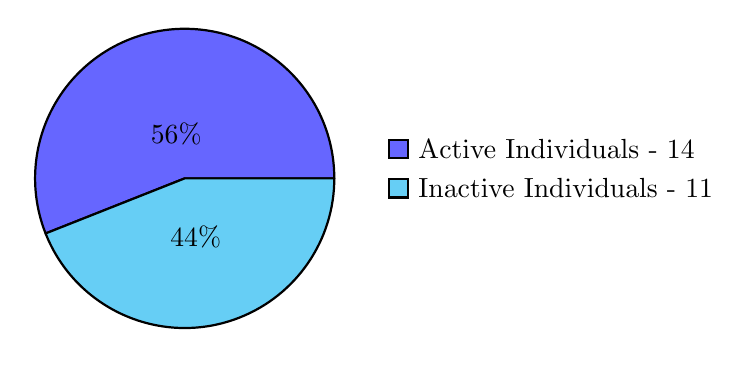
\begin{tikzpicture} 
    \pie[radius = 1.9,text=legend]{56/Active Individuals - 14,44/Inactive Individuals - 11}
\end{tikzpicture}
\end{center}
\subsection{Frequency of Tandem Runs}
We will now see the frequency of tandem runs, in intervals of 5 mins. 
\begin{table}[H]\centering
\scriptsize
\begin{tabular}{lrrr}\toprule
    Slno&Time Intervals &No of tandem runs \\\midrule
1&0-5 &0 \\
2&5-10 &0 \\
3&10-15 &3 \\
4&15-20 &10 \\
5&20-25 &15 \\
6&25-30 &11 \\
7&30-35 &0 \\
8&35-40 &1 \\
\bottomrule
\end{tabular}
\end{table}
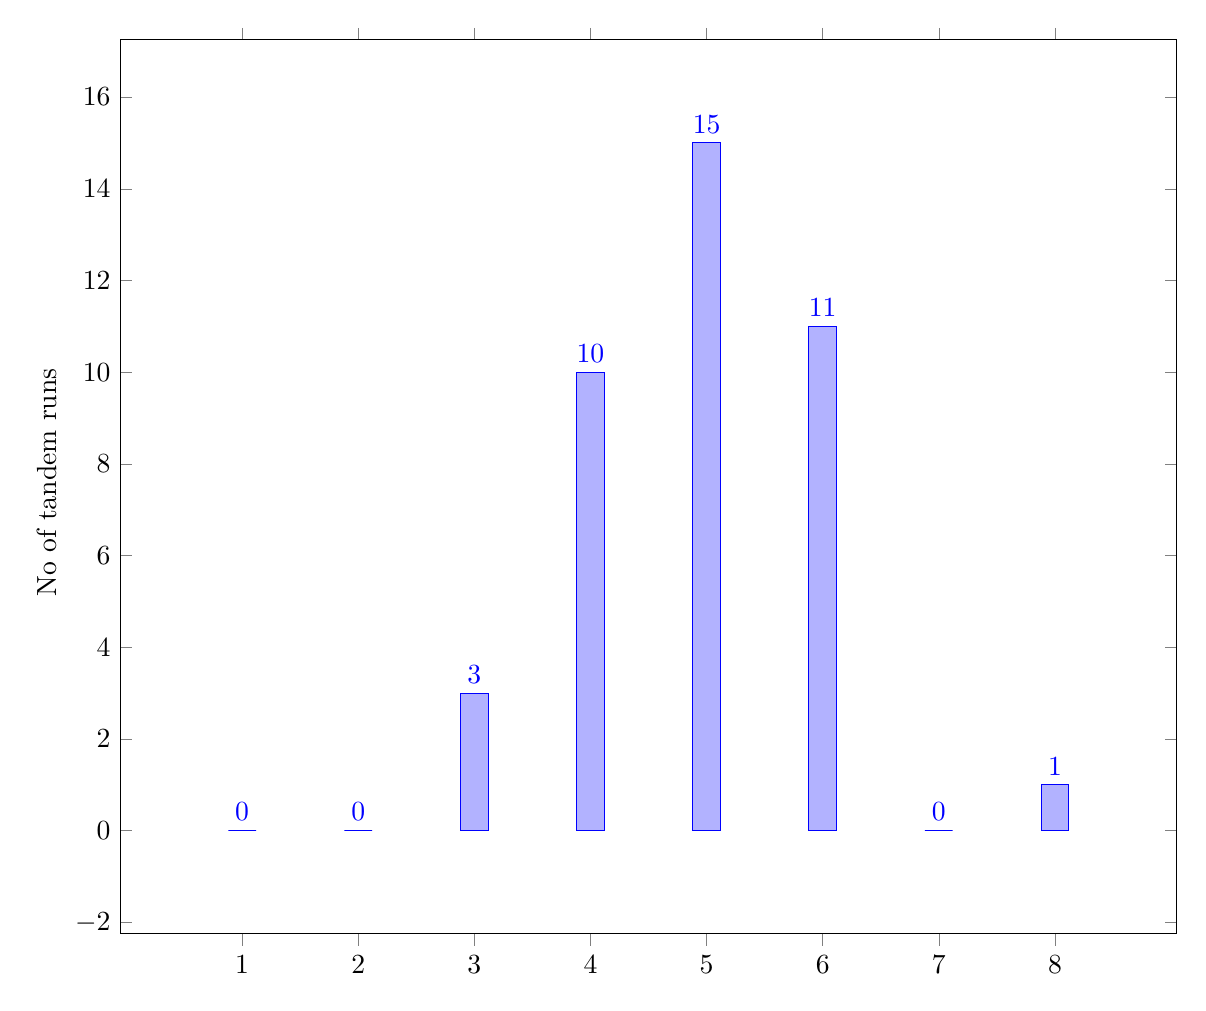
\begin{tikzpicture}
        \begin{axis}  
        [  
            ybar,  
            enlargelimits=0.15,  
            ylabel={\ No of tandem runs}, % the ylabel must precede a # symbol.
            symbolic x coords={1,2,3,4,5,6,7,8}, % these are the specification of coordinates on the x-axis.  
            xtick=data,  
             nodes near coords, % this command is used to mention the y-axis points on the top of the particular bar.  
            nodes near coords align={vertical},  
        ]  
        \addplot coordinates {(1,0) (2,0) (3,3) (4,10) (5,15) (6,11) (7,0) (8,1)};  
      
    \end{axis}  
    \end{tikzpicture}\\
    We can see that the bin with the highest no of tandem runs in 5 i.e. the 20-25 min window in the 
picture.
\section{Limitations}
The limitations of this experiment are:
\begin{enumerate}
  \item We observe the behaviour of ants from a pre recorded video. Here the colours of individual ants are 
      not always distinguished properly. For example, the blue colour painted on the ant was very hard to distinguish from the 
      natural exoskeleton of the ant, causing us to undercount the number of individuals.
      \item The distinction between active and inactive individuals depends heavily on the person performing the experiment.
           I have chosen to take 1 second each back and forth to check if the ants are moving within that time frame. 
           Someone may choose a larger time frame, and someone may choose a shorter time frame with varying results.
           Thus the distinction here between active and inactive individuals is very crude.
           \item Sometimes, tandem runs can get complicated. Ther are atleast two instances throughout the 
               whole video where there have been simultaneuos tandem runs. At around 23 mins, 4 ants perform a chain together and perform tandem runs. 
               However, by definition, tandem runs are defined pairwise. So for those tandem runs that involve more than two ants, we have taken, that the ant 
               immediately in front of some ant acts as the leader of that ant.
\end{enumerate}
\section{Conclusions}
We hereby conclude the experiment with the following results:
\begin{enumerate}
    \item We have identified atleast \textbf{33 unique individuals} from the whole video.
    \item  There have been 10 leaders for all the tandem runs, with \textbf{y-w} being the most efficient ant with the highest no of tandem runs. 
\end{enumerate}
\section{Supplementary}
The raw data collected is attached below.
\end{document}
